\documentclass[12pt]{article}
\usepackage[margin=2.5cm]{geometry}
\usepackage{enumerate}
\usepackage{amsfonts}
\usepackage{amsmath}
\usepackage{fancyhdr}
\usepackage{amsmath}
\usepackage{amssymb}
\usepackage{amsthm}
\usepackage{mdframed}
\usepackage{graphicx}
\usepackage{subcaption}
\usepackage{adjustbox}
\usepackage{listings}
\usepackage{xcolor}
\usepackage{booktabs}
\usepackage[utf]{kotex}
\usepackage{hyperref}

\definecolor{codegreen}{rgb}{0,0.6,0}
\definecolor{codegray}{rgb}{0.5,0.5,0.5}
\definecolor{codepurple}{rgb}{0.58,0,0.82}
\definecolor{backcolour}{rgb}{0.95,0.95,0.92}

\lstdefinestyle{mystyle}{
    backgroundcolor=\color{backcolour},
    commentstyle=\color{codegreen},
    keywordstyle=\color{magenta},
    numberstyle=\tiny\color{codegray},
    stringstyle=\color{codepurple},
    basicstyle=\ttfamily\footnotesize,
    breakatwhitespace=false,
    breaklines=true,
    captionpos=b,
    keepspaces=true,
    numbers=left,
    numbersep=5pt,
    showspaces=false,
    showstringspaces=false,
    showtabs=false,
    tabsize=1
}

\lstset{style=mystyle}

\pagestyle{fancy}
\renewcommand{\headrulewidth}{0.4pt}
\lhead{CSC 373}
\rhead{Worksheet 4 Solution}

\begin{document}
\title{CSC373 Worksheet 4 Solution}
\maketitle

\bigskip

\begin{enumerate}[1.]
    \item

    \bigskip

    \underline{\textbf{Notes:}}

    \bigskip

    \begin{itemize}
        \item \textbf{Vertex}
        \begin{itemize}
            \item Is a fundamental unit of which graphs are formed
            \item Also means node

            \begin{center}
            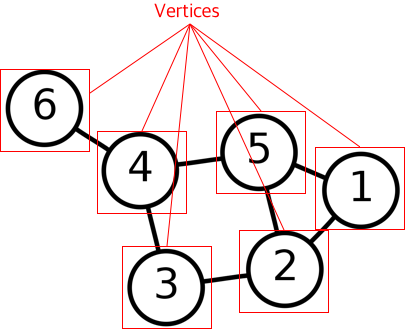
\includegraphics[width=0.4\linewidth]{images/worksheet_4_solution_1.png}
            \end{center}
        \end{itemize}

        \item \textbf{Adjacency-list Representation}
        \begin{itemize}
            \item Associates each vertax in a graph with the collection of its neighbouring vertices or edges
            \item Is represented by $Adj[v]$
            \begin{itemize}
                \item Means all vertices that are neighbour to vertex $v$
                \item In a directed graph, $Adj[v]$ are all out-degree vertices of vertax $v$
            \end{itemize}
        \end{itemize}

        \begin{center}
        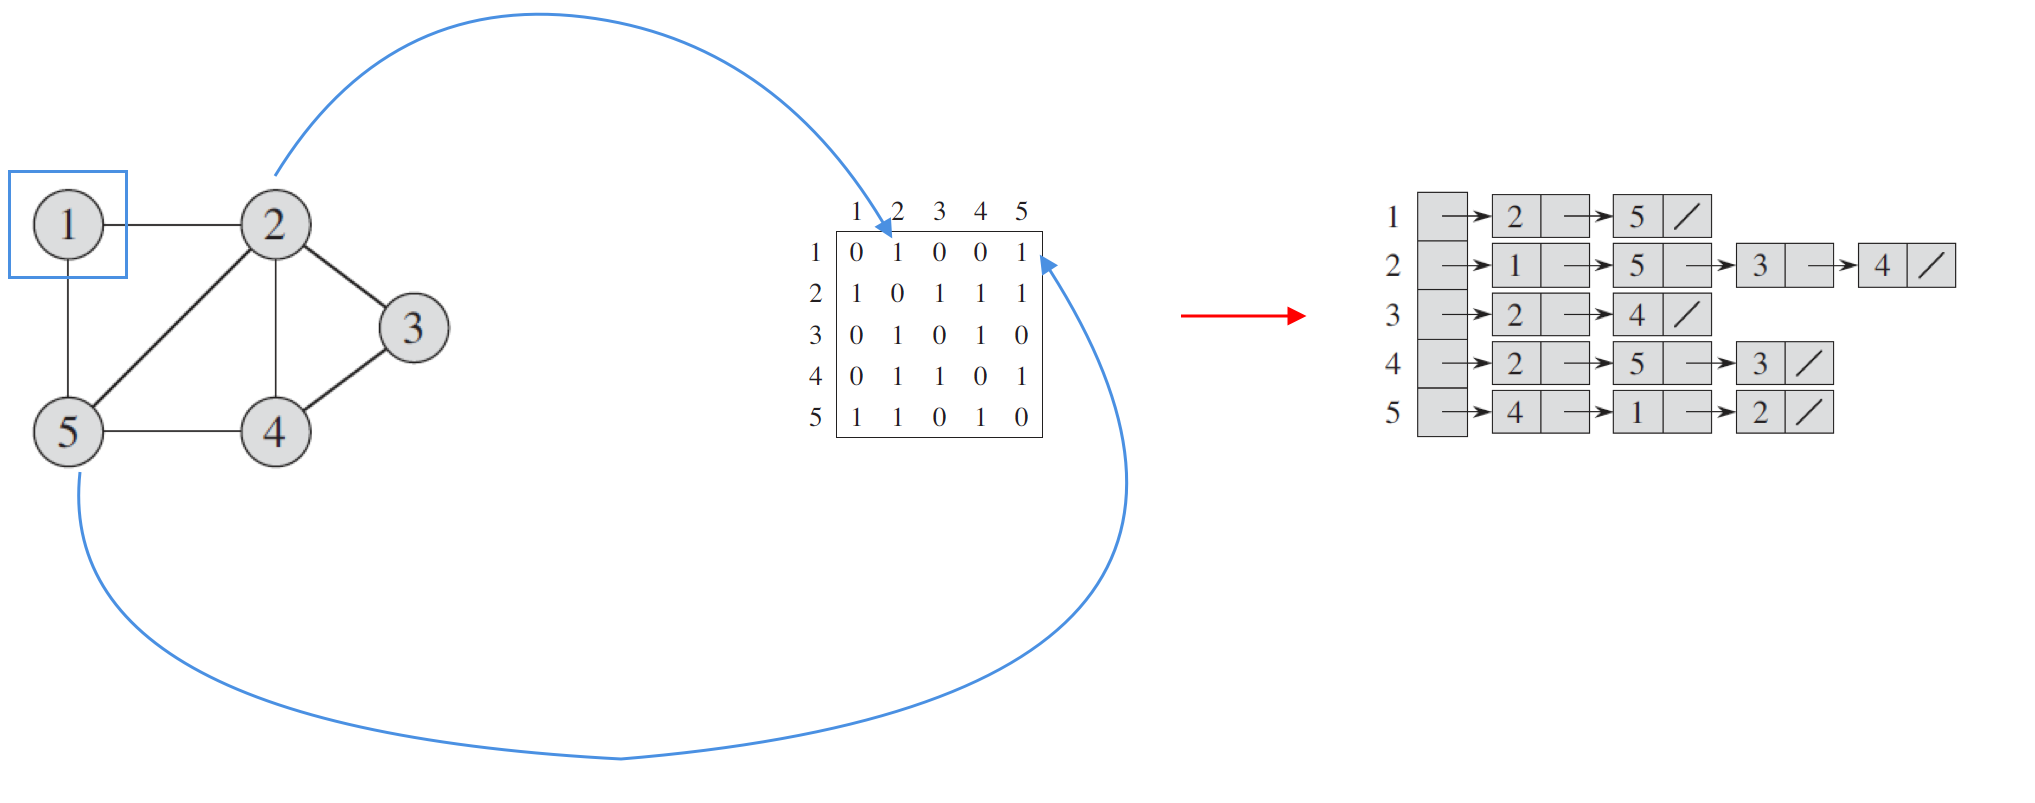
\includegraphics[width=\linewidth]{images/worksheet_4_solution_2.png}
        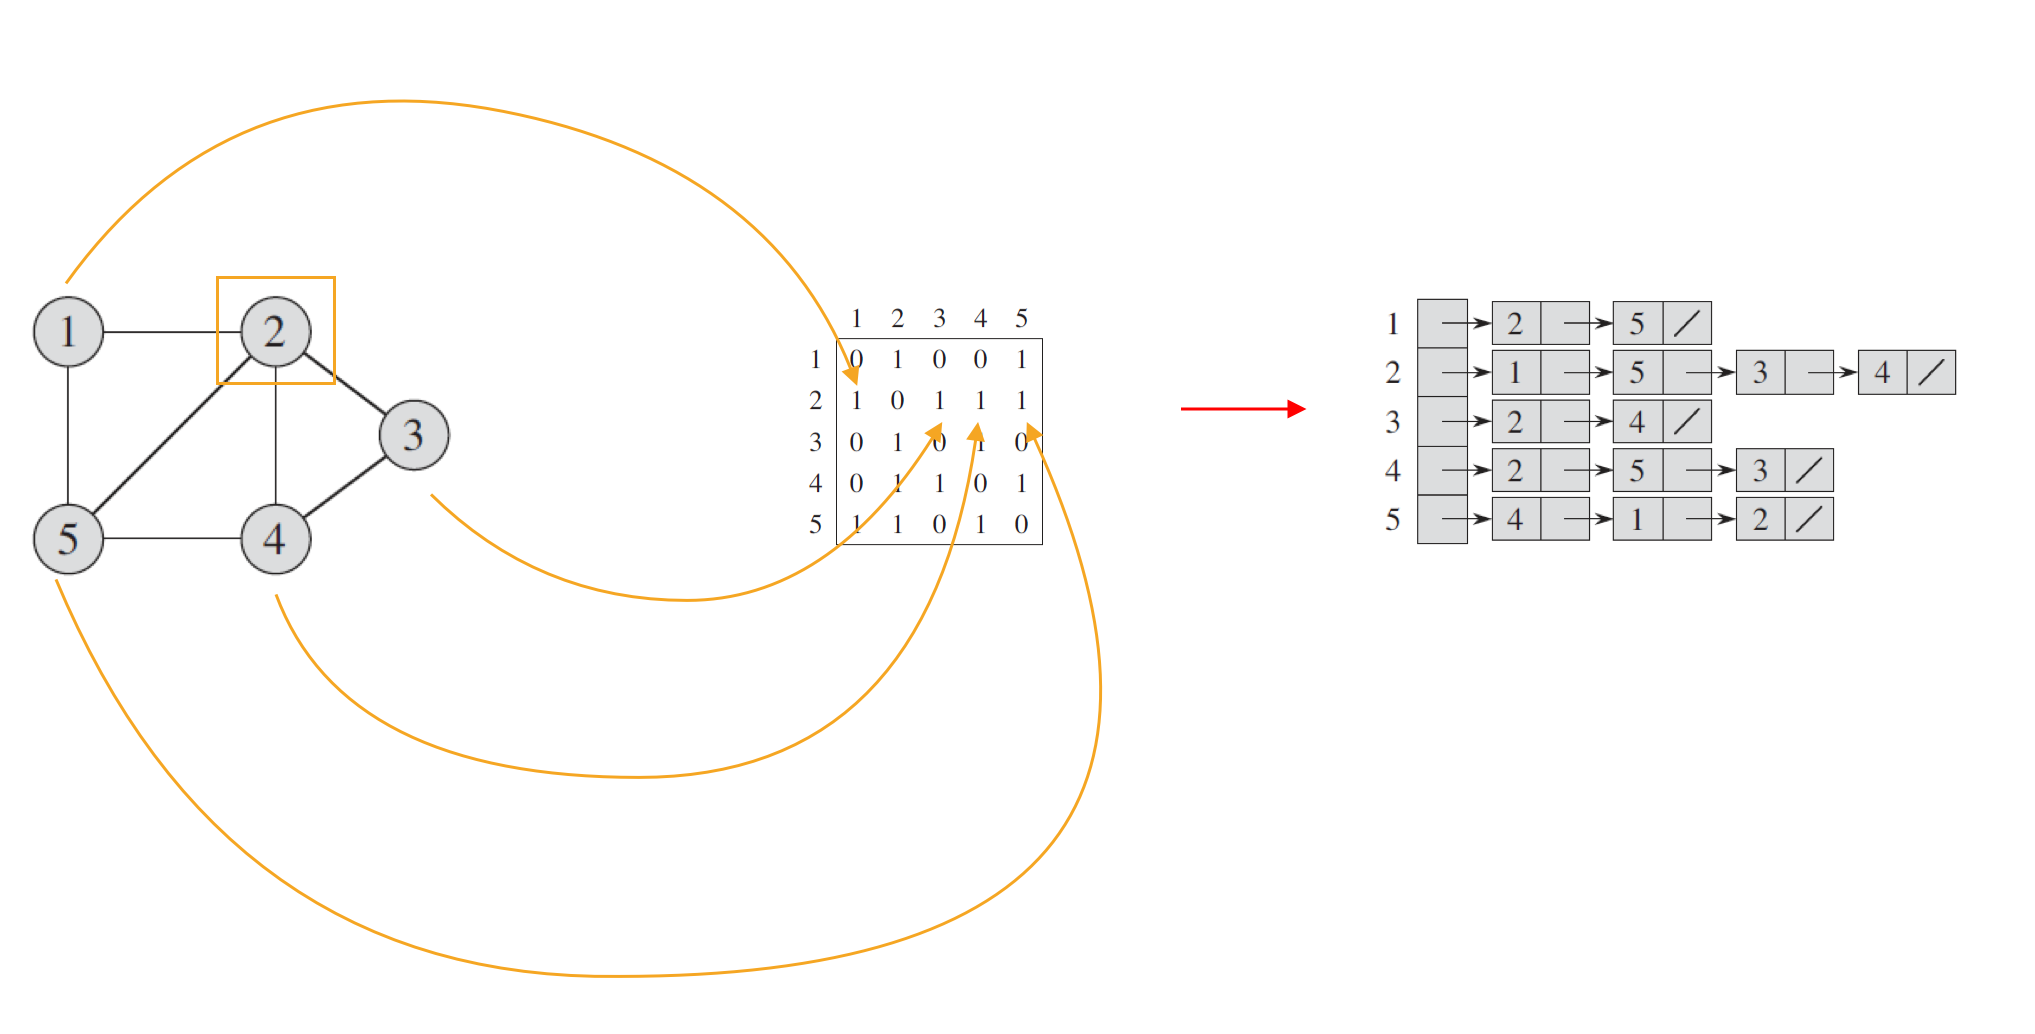
\includegraphics[width=\linewidth]{images/worksheet_4_solution_3.png}
        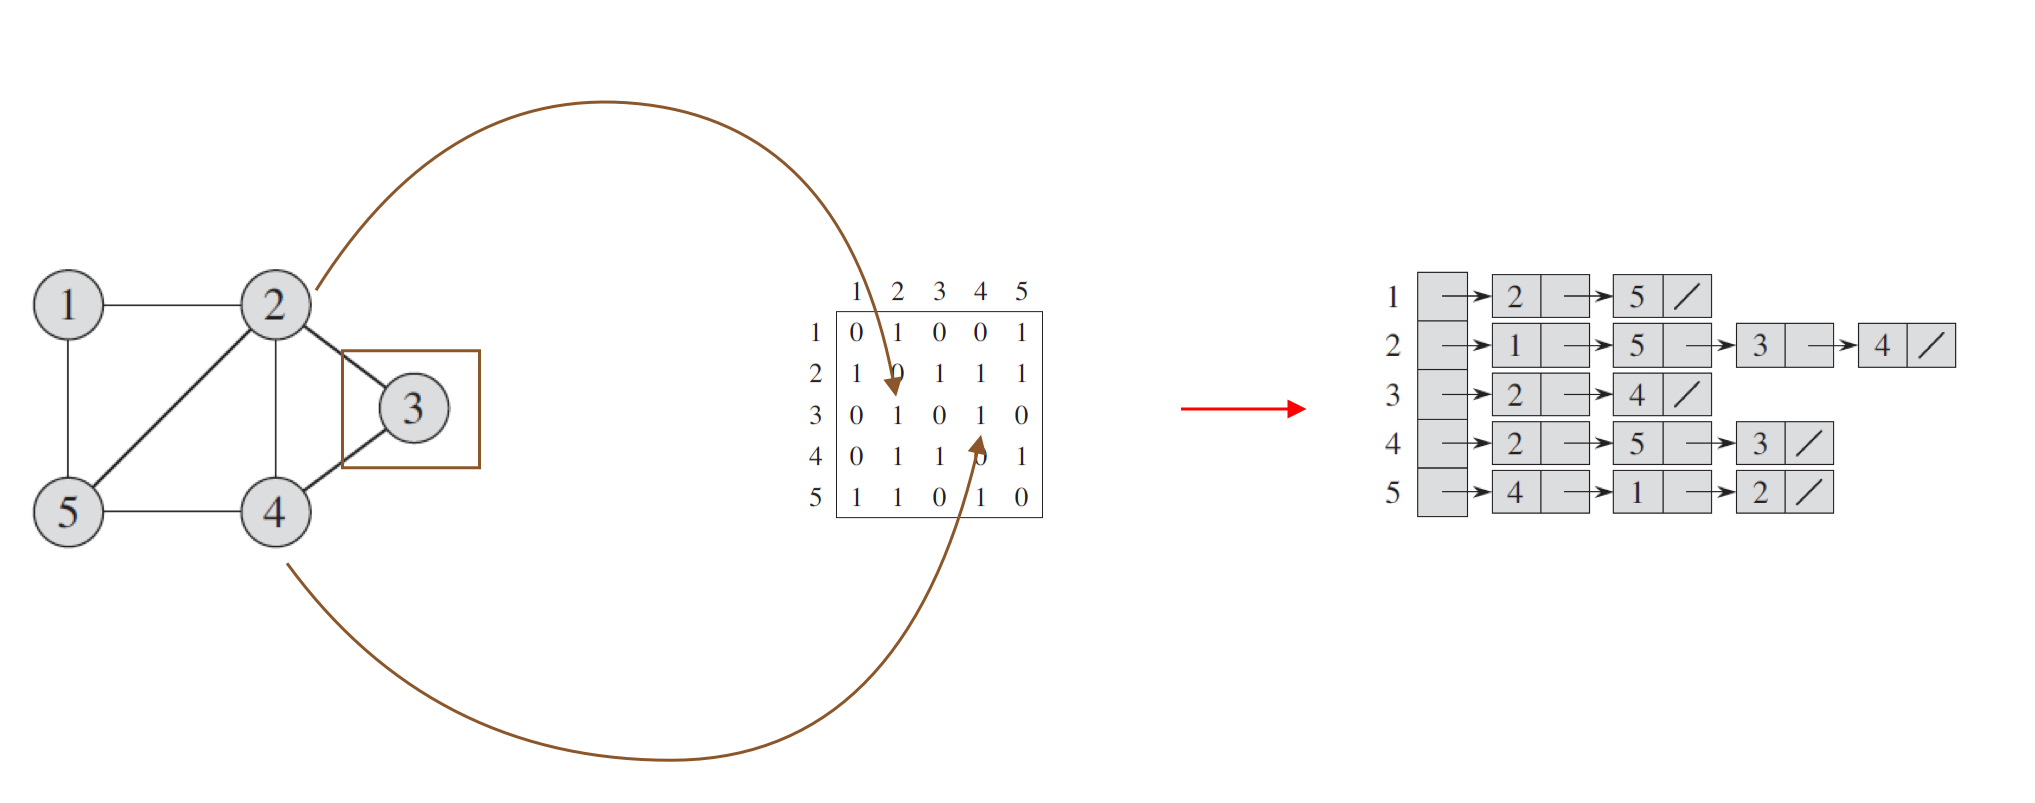
\includegraphics[width=\linewidth]{images/worksheet_4_solution_4.png}
        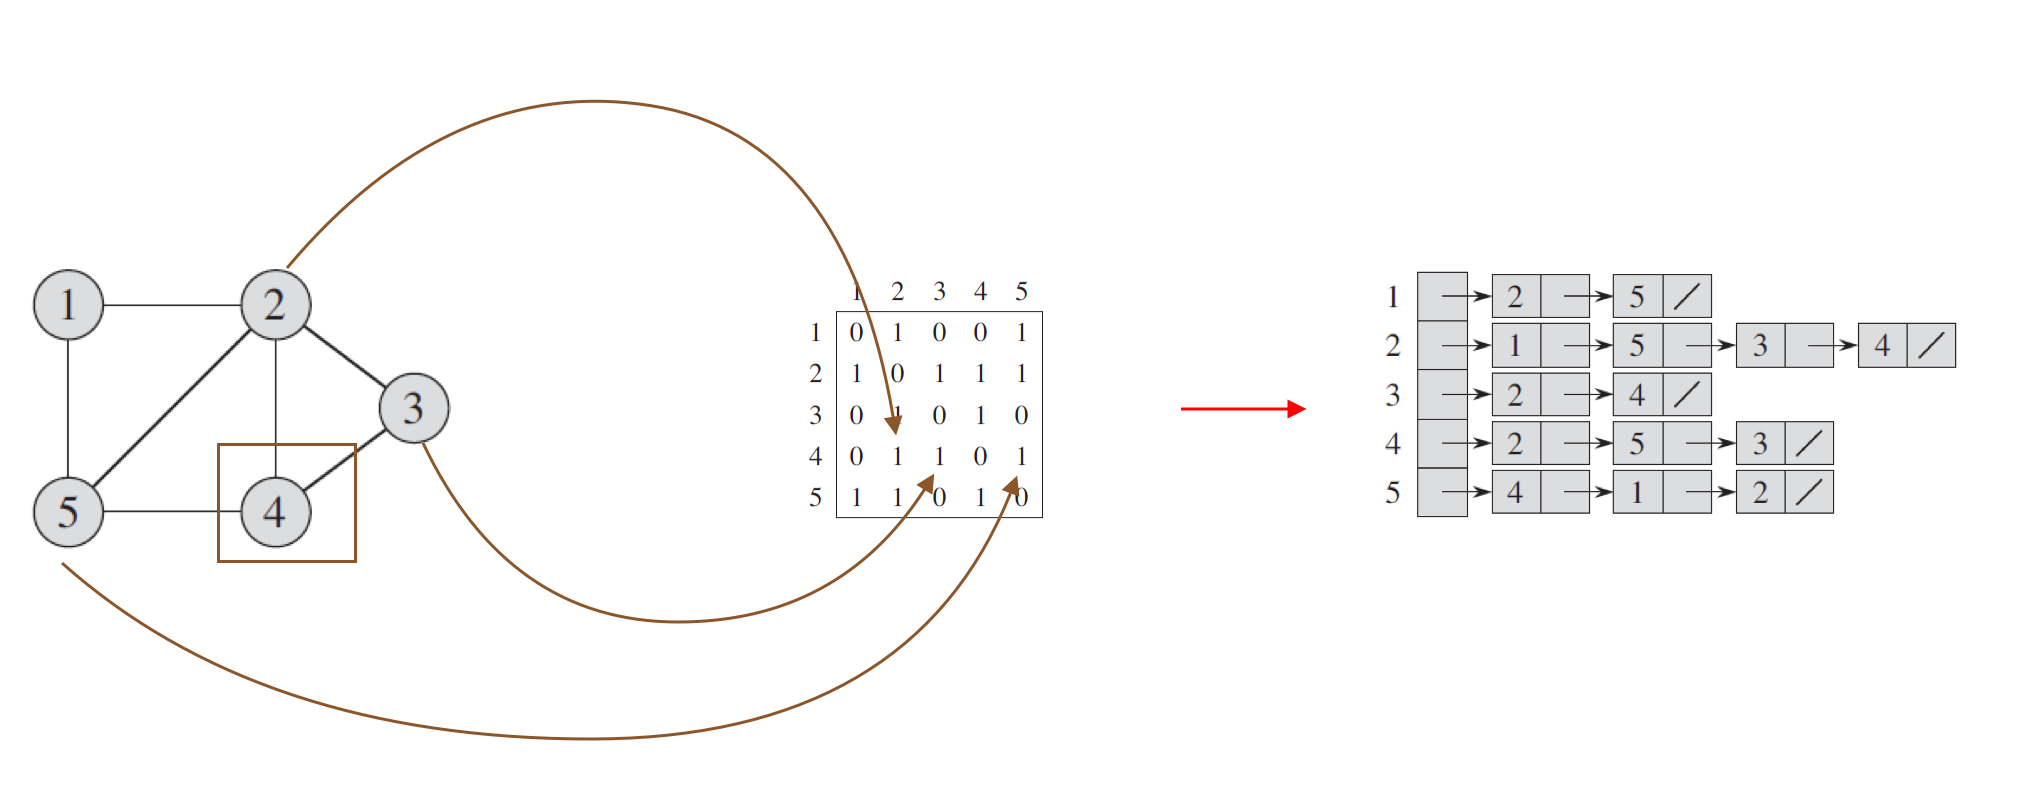
\includegraphics[width=\linewidth]{images/worksheet_4_solution_5.png}
        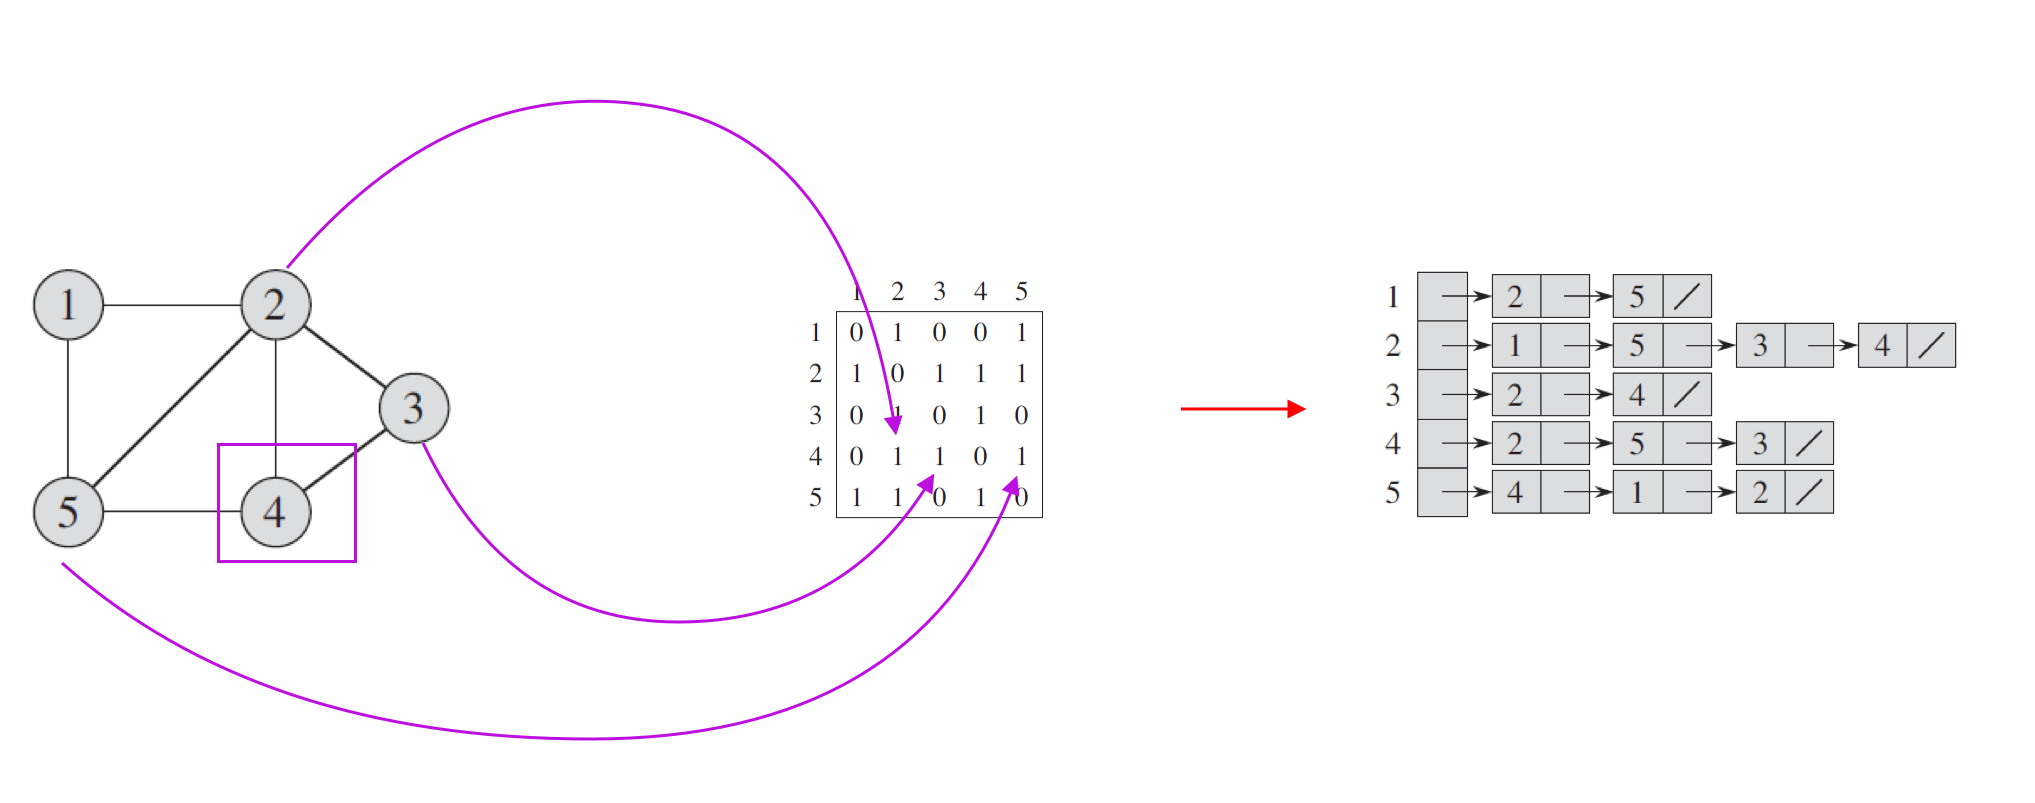
\includegraphics[width=\linewidth]{images/worksheet_4_solution_6.png}
        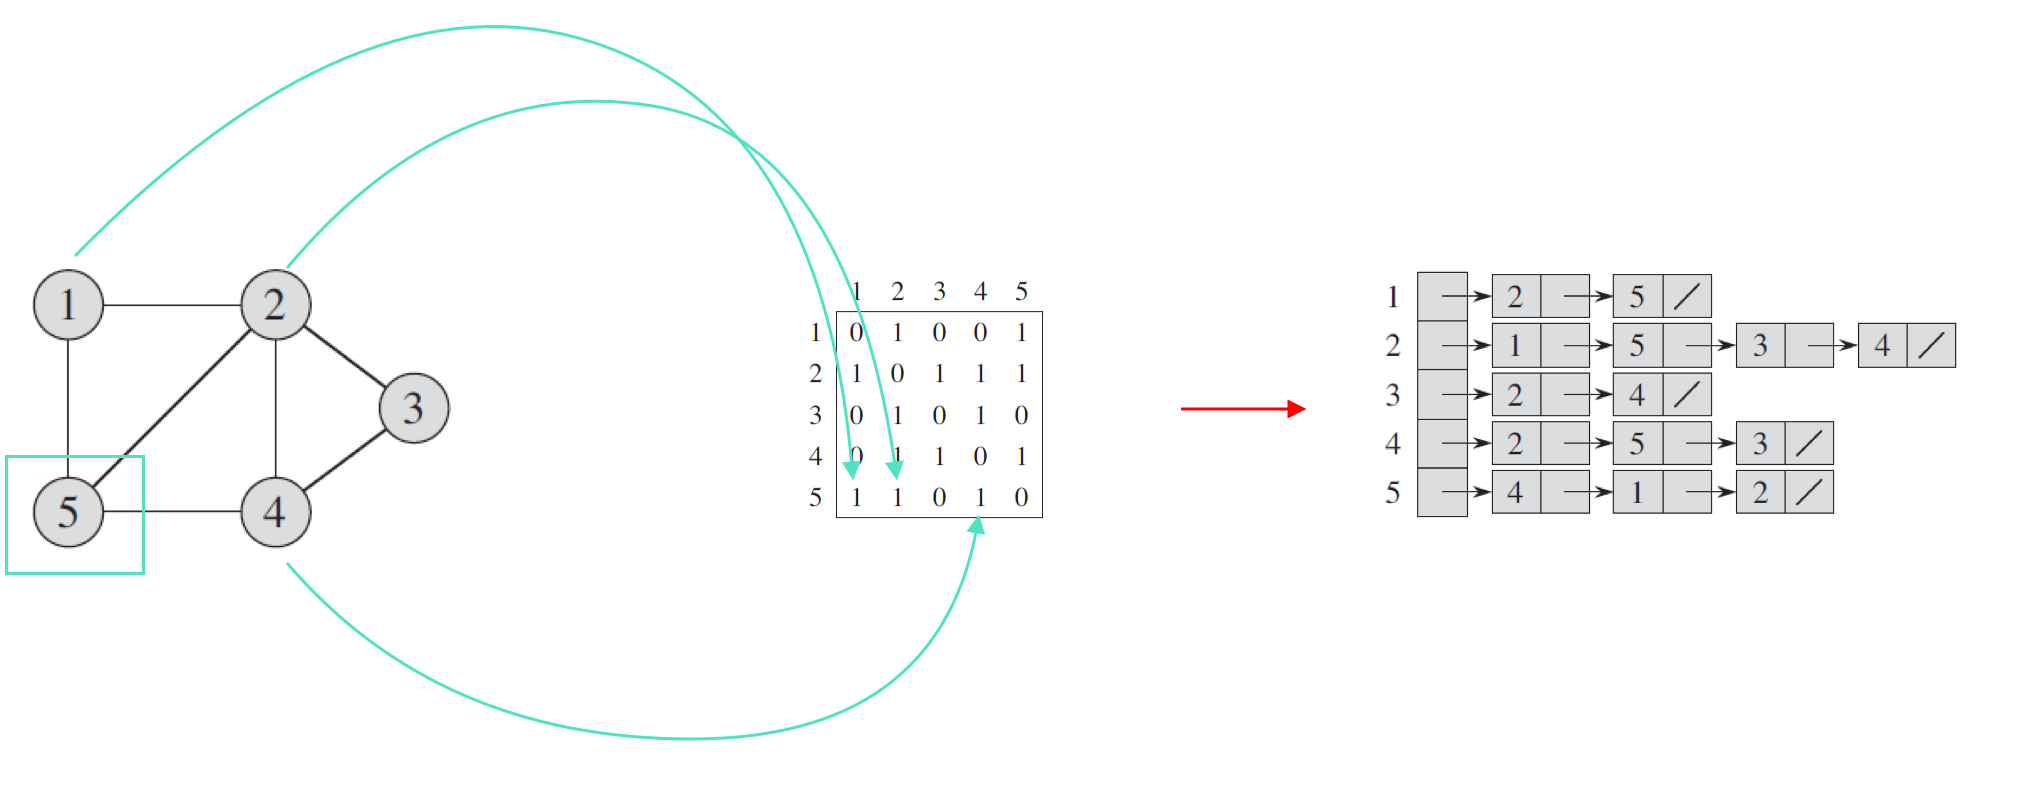
\includegraphics[width=\linewidth]{images/worksheet_4_solution_7.png}
        \end{center}

        \item \textbf{Directed graph}
        \begin{itemize}
            \item Is a graph that is made up of a set of vertices connected by edges,
            where the edges have a direction associated with them

            \begin{center}
            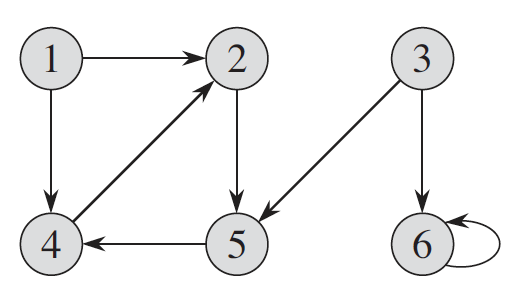
\includegraphics[width=0.4\linewidth]{images/worksheet_4_solution_8.png}
            \end{center}
        \end{itemize}

        \item \textbf{Out-degrees}
        \begin{itemize}
            \item For a directed graph $G=(V(G),E(G))$ and a vertex $x_1 \in V(G)$,
            the Out-Degree of $x_1$ refers to the number of arcs incident from $x_1$.
            That is, the number of arcs directed \underline{away} from the vertex $x_1$.

            \begin{center}
            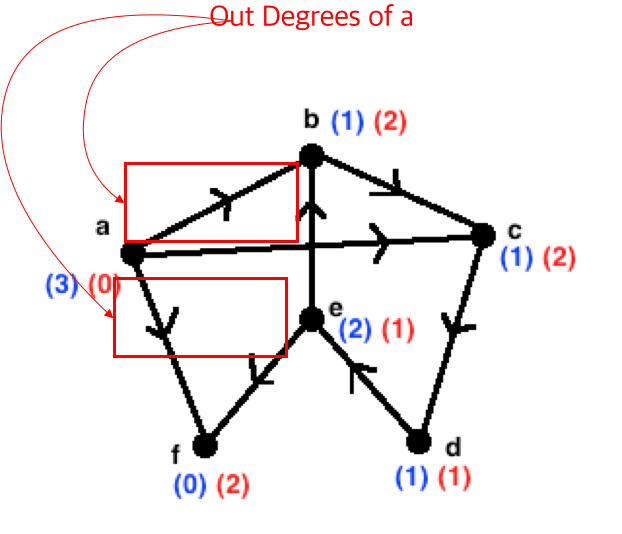
\includegraphics[width=0.4\linewidth]{images/worksheet_4_solution_9.png}
            \end{center}
        \end{itemize}

        \item \textbf{In-degrees}
        \begin{itemize}
            \item For a directed graph $G=(V(G),E(G))$ and a vertex $x_1 \in V(G)$,
            the In-Degree of $x_1$ refers to the number of arcs incident to $x_1$.
            That is, the number of arcs directed \underline{towards} the vertex $x_1$.

            \begin{center}
            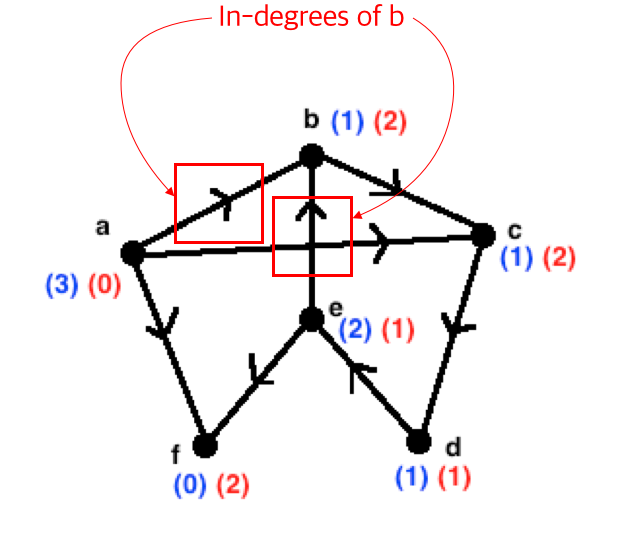
\includegraphics[width=0.4\linewidth]{images/worksheet_4_solution_10.png}
            \end{center}
        \end{itemize}
    \end{itemize}

\end{enumerate}

\end{document}